\documentclass[12pt,letterpaper]{exam}
\usepackage[lmargin=1in,rmargin=1in,tmargin=1in,bmargin=1in]{geometry}
\usepackage{../style/exams}

% -------------------
% Course & Exam Information
% -------------------
\newcommand{\course}{MAT 108: Exam 2}
\renewcommand{\term}{Spring -- 2022}
\newcommand{\examdate}{04/13/2022}
\newcommand{\timelimit}{85 Minutes}

\setbool{hideans}{false} % Student: True; Instructor: False

% -------------------
% Content
% -------------------
\begin{document}

\examtitle
\instructions{Write your name on the appropriate line on the exam cover sheet. This exam contains \numpages\ pages (including this cover page) and \numquestions\ questions. Check that you have every page of the exam. Answer the questions in the spaces provided on the question sheets. Be sure to answer every part of each question and show all your work. If you run out of room for an answer, continue on the back of the page --- being sure to indicate the problem number.} 
\scores
\bottomline
\newpage

% ---------
% Questions
% ---------
\begin{questions}

% Question 1
\newpage
\question Consider the function $f(x, y)= 3x - 2y$ on the `crooked house' feasible set shown below. 

	\[
	\fbox{
	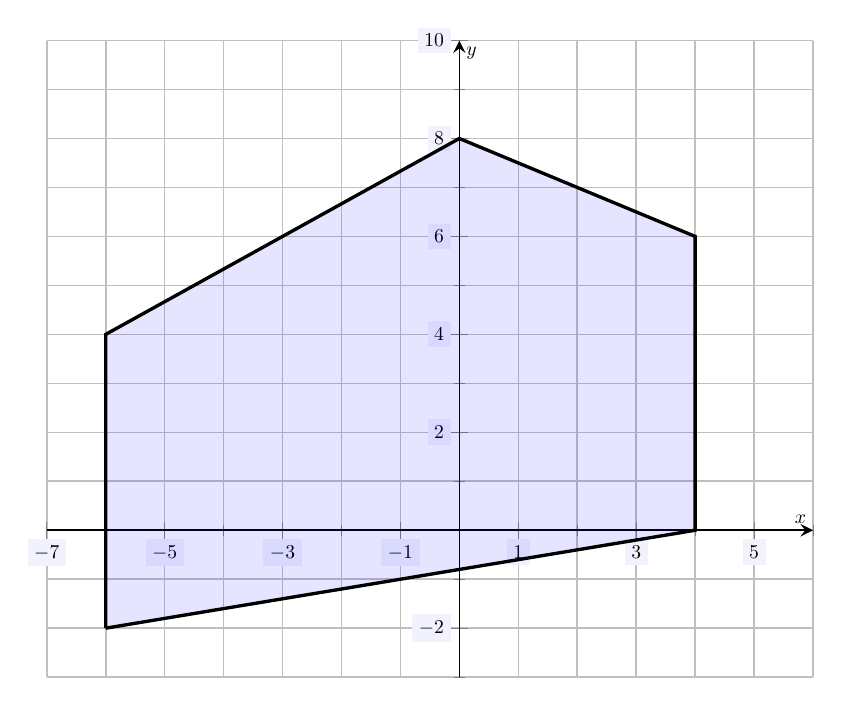
\begin{tikzpicture}[scale=1.42,every node/.style={scale=0.5}]
	\begin{axis}[
	grid=both,
	axis lines=middle,
	ticklabel style={fill=blue!5!white},
	xmin= -7, xmax=6,
	ymin= -3, ymax=10,
	xtick={-7,-5,...,7},
	ytick={-2,0,...,10},
	minor tick = {-10,-9,...,10},
	xlabel=\(x\),ylabel=\(y\),
	]
	\draw[line width=0.01cm,fill= blue,opacity=0.1] (-6,-2) -- (-6,4) -- (0,8) -- (4,6) -- (4,0) -- (-6,-2);
	\draw[line width=0.03cm] (-6,-2) -- (-6,4) -- (0,8) -- (4,6) -- (4,0) -- (-6,-2);
	\end{axis}
	\end{tikzpicture}
	}
	\] \pspace

\begin{parts}
\part[3] Explain why the Fundamental Theorem of Linear Programming applies to the function $f(x, y)$ on the feasible set shown above. \pspace

{\itshape Because the function is linear, the feasible set is nonempty, and the feasible set is bounded, the Fundamental Theorem of Linear Programming applies to the function $f(x, y)$ on the feasible set shown above.} \pvspace{0.87cm}


\part[7] Use the Fundamental Theorem of Linear Programming to find $\max f(x, y)$ and $\min f(x, y)$ on the feasible set shown above. \pspace

{\itshape The Fundamental Theorem of Linear Programming states that the maximum and minimum values of $f(x, y)$ exist on the feasible set shown above. Moreover, the max and min must occur at a corner point for the feasible set. 
	\begin{table}[!ht]
	\centering
	\begin{tabular}{c | l}
	\textit{Corner Point} & $f(x, y)$ \\ \hline
	$(-6, 4)$ & $3(-6) - 2(4)= -26$ \\
	$(0, 8)$ & $3(0) - 2(8)= -16$ \\
	$(4, 6)$ & $3(4) - 2(6)= 0$ \\
	$(4, 0)$ & $3(4) - 2(0)= 12$ \\
	$(-6, -2)$ & $3(-6) - 2(-2)= -14$
	\end{tabular}
	\end{table} \par
Therefore, the maximum value is $12$ and occurs at $(4, 0)$ while the minimum value is $-26$ and occurs at $(-6, 4)$. 
}
\end{parts}



% Question 2
\newpage
\question[10] Find the initial simplex tableau for the linear programming problem shown below.
	\[
	\max z= 3x_1 - 5x_2 + 2x_3
	\]
	\[
	\left\{
	\begin{aligned}
	x_1 + 7x_2 - 3x_3 &\leq 10 \\
	2x_1 + 10x_3 &\leq 12 \\
	x_1 - x_2 + 5x_3 &\leq 7 \\
	x_1 - 4x_2 - 9x_3 &\geq -8
	\end{aligned} \right.
	\]
	\[
	x_1,\, x_2,\, x_3 \geq 0
	\] \pspace

{\itshape Moving everything to the left side in the equality $z= 3x_1 - 5x_2 + 2x_3$, we have $z - 3x_1 + 5x_2 - 2x_3= 0$. Observe that for the inequalities to be in standard form for a maximization problem, we need the fourth inequality to be multiplied by $-1$ on both sides (so that we have $\leq$), which gives us the following inequalities: 
	\[
	\left\{
	\begin{aligned}
	x_1 + 7x_2 - 3x_3 &\leq 10 \\
	2x_1 + 10x_3 &\leq 12 \\
	x_1 - x_2 + 5x_3 &\leq 7 \\
	-x_1 + 4x_2 + 9x_3 &\leq 8
	\end{aligned} \right.
	\] 

Introducing slack variables into each inequality and aligning the equalities, we have\dots \pspace

\begin{table}[!ht]
\centering
\begin{tabular}{rrrrrrrrrrrrrrl}
	& $x_1$    & $+$ & $7x_2$  & $+$ & $-3x_3$  & $+$ & $1s_1$ &        &              &        &              &        &              & $= 10$ \\
	& $2x_1$  & $+$ & $0x_2$  & $+$ & $10x_3$ &        &              & $+$ & $1s_2$ &        &              &        &              & $= 12$ \\
	& $x_1$    & $+$ & $-1x_2$ & $+$ & $5x_3$   &        &              &        &              & $+$ & $1s_3$ &        &              & $= 7$ \\
	& $-x_1$    & $+$ & $4x_2$ & $+$ & $9x_3$  &        &              &        &              &        &              & $+$ & $1s_4$ & $= 8$ \\
$z$ 	& $-3x_1$ & $+$ & $5x_2$  & $+$ & $-2x_3$  &        &              &        &              &        &              &        &              & $= 0$ 
\end{tabular}
\end{table} \pspace

This gives us the following initial simplex tableau: \pspace
	\begin{table}[!ht]
	\centering
	\begin{tabular}{rrrrrrr|r}
	$1$ & $7$ & $-3$ & $1$ & $0$ & $0$ & $0$ & $10$ \\
	$2$ & $0$ & $10$ & $0$ & $1$ & $0$ & $0$ & $12$ \\
	$1$ & $-1$ & $5$ & $0$ & $0$ & $1$ & $0$ & $7$ \\
	$-1$ & $4$ & $9$ & $0$ & $0$ & $0$ & $1$ & $8$ \\ \hline
	$-3$ & $5$ & $-2$ & $0$ & $0$ & $0$ & $0$ & $0$ 
	\end{tabular}
	\end{table}
}



% Question 3
\newpage
\question Below is the initial simplex tableau associated to a standard maximization problem. 
	\begin{table}[!ht]
	\centering
	\begin{tabular}{rrrrr|r}
	$2$ & $3$ & $1$ & $0$ & $0$ & $20$ \\
	$-1$ & {\large \textcircled{\small$7$}} & $0$ & $1$ & $0$ & $15$ \\
	$4$ & $1$ & $0$ & $0$ & $1$ & $30$ \\ \hline
	$9$ & $-5$ & $0$ & $0$ & $0$ & $0$ 
	\end{tabular}
	\end{table}

\begin{parts}
\part[1] How many inequalities were in the original problem? \pvspace{0.4cm}

{\itshape There are four rows in the tableau. The last row corresponds to the function. The other three rows then correspond to inequalities. Therefore, there are three inequalities.} \pvspace{0.4cm}

\part[1] How many slack variables are there? \pvspace{0.65cm}

{\itshape A slack variable is introduced in each inequality. By (a), we know there are three inequalities. Therefore, there are three slack variables.} \pvspace{0.65cm}

\part[1] How many decision variables are there? \pvspace{0.45cm}

{\itshape The last column corresponds to the `solution vector.' Every other column corresponds to a variable---either a decision variable or a slack variable. By (b), we know there are three slack variables. Therefore, there are two decision variables.} \pvspace{0.45cm}

\part[3] If one were to perform the simplex algorithm, circle the initial pivot position. \pvspace{0.2cm}

{\itshape We choose the column with the most negative entry in the bottom row. This is the second column. We then choose the entry with `the smallest positive ratio.' We have ratios $20/3 \approx 6.666$, $15/7 \approx 2.143$, $30/1= 30$. Therefore, we choose the $7$ entry as our pivot position.} \pvspace{0.2cm}

\part[4] Write the original maximization problem. 

	\[
	\max z= -9x_1 + 5x_2
	\]
	\[
	\left\{
	\begin{aligned}
	2x_1 + 3x_2&\leq 20 \\
	-x_1 + 7x_2&\leq 15 \\
	4x_1 + x_2&\leq 30
	\end{aligned} \right.
	\]
	\[
	x_1,\, x_2 \geq 0
	\]
\end{parts}



% Question 4
\newpage
\question[10] Below is the final simplex tableau from the simplex algorithm used to solve a standard maximization problem. Find the solution along with the maximum value. Be sure to indicate the value of all variables involved. 
	\begin{table}[!ht]
	\centering
	\begin{tabular}{rrrrrrr|r}
	$0$ & $1$ & $-1.21$ & $0.05$ & $0.21$ & $0$ & $-0.05$ & $5.26$ \\
	$0$ & $0$ & $3.66$ & $16.21$ & $0.34$ & $1$ & $0.29$ & $321.05$ \\
	$1$ & $0$ & $0.82$ & $0.42$ & $0.18$ & $0$ & $0.08$ & $42.11$ \\ \hline
	$0$ & $0$ & $29.44$ & $99.39$ & $35.56$ & $0$ & $2.21$ & $4218.95$ \\
	\end{tabular}
	\end{table} \pspace

{\itshape We know there are $4 - 1= 3$ slack variables and $8 - 1 - 3= 4$ decision variables. We rewrite the table, carefully labeling the columns and indicating the basic variables. This gives us the following table:
	\begin{table}[!ht]
	\centering
	\begin{tabular}{rrrrrrrrl}
	\footnotesize$x_1$ & \footnotesize$x_2$ & \footnotesize$x_3$ & \footnotesize$x_4$ & \footnotesize$s_1$ & \footnotesize$s_2$ & \footnotesize$s_3$ \\
	$0$ & $1$ & $-1.21$ & $0.05$ & $0.21$ & $0$ & \multicolumn{1}{r|}{$-0.05$} & $5.26$ & \footnotesize$x_2$ \\
	$0$ & $0$ & $3.66$ & $16.21$ & $0.34$ & $1$ & \multicolumn{1}{r|}{$0.29$} & $321.05$ & \footnotesize$s_2$ \\
	$1$ & $0$ & $0.82$ & $0.42$ & $0.18$ & $0$ & \multicolumn{1}{r|}{$0.08$} & $42.11$ & \footnotesize$x_1$ \\ \cline{1-8}
	$0$ & $0$ & $29.44$ & $99.39$ & $35.56$ & $0$ & \multicolumn{1}{r|}{$2.21$} & $4218.95$ \\
	\end{tabular}
	\end{table} \par
We then see that the solution is\dots
	\[
	(x_1,\, x_2,\, x_3,\, x_4,\, s_1,\, s_2,\, s_3)= (42.11,\, 5.26,\, 0,\, 0,\, 0,\, 321.05,\, 0)
	\]
From the bottom-right entry of the tableau, we see that the maximum value of the function is $4218.95$. 
}



% Question 5
\newpage
\question[10] Below is a linear programming minimization problem. Find the associated dual problem. 
	\[
	\min w= 5x_1 + 4x_2
	\]
	\[
	\left\{
	\begin{aligned}
	4x_1 - x_2 &\geq 8 \\
	x_1 + 5x_2&\leq -12
	\end{aligned} \right.
	\]
	\[
	x_1,\, x_2 \geq 0
	\] \pspace

{\itshape First, note that the problem is not in standard form. We multiply both sides of the second inequality by $-1$ to obtain\dots \pspace
	\[
	\left\{
	\begin{aligned}
	4x_1 - x_2 &\geq 8 \\
	-x_1 - 5x_2&\geq 12
	\end{aligned} \right.
	\] \pspace
Writing the matrix associated to the inequalities and the function, we have\dots \pspace
	\[
	A= 
	\begin{pmatrix}
	4 & -1 & 8 \\
	-1 & -5 & 12 \\
	5 & 4 & 0 
	\end{pmatrix}
	\] \pspace
Taking the transpose of this matrix, we have\dots \pspace
	\[
	A^T= 
	\begin{pmatrix}
	4 & -1 & 5 \\
	-1 & -5 & 4 \\
	8 & 12 & 0 
	\end{pmatrix}
	\] \pspace
The maximization problem associated to this matrix is\dots \pspace
	\[
	\max z= 8y_1 + 12y_2
	\]
	\[
	\left\{
	\begin{aligned}
	4y_1 - y_2&\leq 5 \\
	-y_1 - 5y_2&\leq 4
	\end{aligned} \right.
	\]
	\[
	y_1,\, y_2 \geq 0
	\] 
}
	


% Question 6
\newpage
\question Sal Ami wants to start offering weekly classes on fancy party hosting to stir up business for his delicatessen. To pay for some of the additions he will make to his shop, he takes out a \$2,500 loan from the bank and is charged a 5.8\% discount on the 6-month loan. \pspace

\begin{parts}
\part[3] What is the discount on the loan? \pvspace{1.4cm}

	\[
	D= Mrt= 2500(0.058) \left( \frac{6}{12} \right)= \$72.50
	\] \pvspace{1.4cm}

\part[2] What are the maturity and proceeds? \pvspace{1.5cm}

{\itshape The maturity is the original loan amount before the discount. Therefore, the maturity is \$2,500. The proceeds are the monies received after the loan is discounted. Therefore, the proceeds are $\$2,500 - \$72.50= \$2,427.50$.} \pvspace{1.5cm}


\part[2] What is Ami's effective interest rate? \pvspace{1.4cm}

	\[
	r_{\text{eff}}= \dfrac{r}{1 - rt}= \dfrac{0.058}{1 - 0.058 \cdot \frac{6}{12}}= \dfrac{0.058}{0.971}= 0.0597= 5.97\%
	\] \pvspace{1.4cm}

\part[3] How much does Sal pay on the loan in total? \pvspace{0.4cm}

{\itshape At the end of the six months, Sal repays the full loan of \$2,500, as he has already paid the interest (discount) of \$72.50 up-front. Therefore, he pays $\$2500 + \$72.50= \$2,572.50$ in total.}
\end{parts}



% Question 7
\newpage
\question Bill Goulding is saving to purchase his dream food truck---Lord of the Fries. He places \$9,700 in an account which earns 6.1\% annual interest, compounded monthly. \pspace 
	
\begin{parts}
\part[3] How much is in this account after 7~years? \pvspace{2cm}

	\[
	F= P \left( 1 + \dfrac{r}{k} \right)^{kt}= 9700 \left( 1 + \dfrac{0.061}{12} \right)^{12 \cdot 7}= 9700(1.5309958) \approx \$14,850.66
	\] \pvspace{2cm}

\part[4] How long until this account has \$20,000? \pvspace{2cm}

	\[
	t= \dfrac{\ln(F/P)}{k \ln\left( 1 + \dfrac{r}{k} \right)}= \dfrac{\ln(20000/9700)}{12 \ln\left( 1 + \dfrac{0.061}{12} \right)}= \dfrac{0.723606}{0.0608455}= 11.89 \text{ years}
	\] \pvspace{2cm}

\part[3] What is the effective yearly interest rate for this account? \pvspace{2cm}

	\[
	r_{\text{eff}}= \left(1 + \dfrac{r}{k} \right)^k - 1= \left(1 + \dfrac{0.061}{12} \right)^{12} - 1= 1.06273 - 1= 0.06273 \approx 6.27\%
	\]
\end{parts}



% Question 8
\newpage
\question  Lon Moore is making some purchases to expand his landscaping business. Given the current number of clients and how much he charges, he knows that he will have around \$6,000 in capital at the end of 5~years. However, he needs the money now. \pspace

\begin{parts}
\part[3] If he takes out a loan now at 4.8\% annual interest, compounded continuously, what is the maximum amount he can take out for the loan initially so that he can pay it off at the end of 5~years? \pvspace{2.1cm}

	\[
	P= \dfrac{F}{e^{rt}}= \dfrac{6000}{e^{0.048 \cdot 5}}= \dfrac{6000}{1.27125} \approx \$4,719.77
	\] \pvspace{2.1cm}

\part[3] What is the effective yearly interest rate on this loan? \pvspace{2cm}

	\[
	r_{\text{eff}}= e^r - 1= e^{0.048} - 1= 1.04917 - 1= 0.04917 \approx 4.92\%
	\] \pvspace{2cm}

\part[4] If he fails to pay off the loan at the end of the 5~years, how much longer after that until the total amount he owes is \$8,000? \pvspace{1.8cm}

{\itshape
	\[
	t= \dfrac{\ln(F/P)}{r}= \dfrac{\ln(8000/6000)}{0.048}= \dfrac{0.287682}{0.048}= 5.993 \approx 6 \text{ years}
	\] \pspace
Therefore, he will owe \$8,000 in a total of 6~years, which is one year after the fifth year. He will then owe \$8,000 in one additional year.}
\end{parts}



% Question 9
\newpage
\question[10] Annita MacDonald and her fianc\'e Ronald Berger are saving for their wedding and honeymoon. [Annita plans on hyphenating her name after marriage.] Their wedding will be in two and a half years. For the next 26~months, they will make monthly payments of \$270 into an account that earns 6.3\% annual interest, compounded monthly. How much will be in the account at the end of the twenty-six months? \pvspace{1cm}

{\itshape
	\[
	\begin{aligned}
	i_p&= \dfrac{r}{k}= \dfrac{0.063}{12}= 0.00525 \\[1cm]
	s_{\actuarialangle{n\,}\, i_p}&= s_{\actuarialangle{26\,}\, 0.00525}= \dfrac{(1 + 0.00525)^{26} - 1}{0.00525}= \dfrac{0.145846}{0.00525}= 27.7801 \\[1cm]
	F&= R\, s_{\actuarialangle{n\,}\, i_p}= 270(27.7801)= 7500.6342 \approx \$7,500.63
	\end{aligned}
	\] \pvspace{0.4cm}
Therefore, the account will have \$7,500.63 after the 26~months. 
}



% Question 10
\newpage
\question Jontra Volta is has recently purchased a condo in Miami. He takes out a \$265,000 mortgage at an annual interest rate of 5.7\%, compounded monthly. Mr. Volta will make monthly payments for the full term of the mortgage, which will be 20~years. \pspace
	
\begin{parts}
\part[4] What are the monthly payments?

{\itshape
	\[
	\begin{aligned}
	i_p&= \dfrac{r}{k}= \dfrac{0.057}{12}= 0.00475 \\[0.3cm]
	n&= kt= 12 \cdot 20= 240 \\[0.5cm]
	a_{\actuarialangle{n\,}\,i_p}&= a_{\actuarialangle{240\,}\,0.00475}= \dfrac{1 - (1 + 0.00475)^{-240}}{0.00475}= \dfrac{0.679317}{0.00475} \approx 143.0140283 \\[0.3cm]
	R&= \dfrac{P}{a_{\actuarialangle{n\,}\,i_p}}= \dfrac{265000}{143.0140283}= 1852.9651 \approx \$1,852.97
	\end{aligned}
	\]
The monthly payments are \$1,852.97.} \pvspace{0.2cm}

\part[4] After 10~years, how much does he still owe on the loan? 

{\itshape
	\[
	\begin{aligned}
	i_p&= \dfrac{r}{k}= \dfrac{0.057}{12}= 0.00475 \\
	n&= kt= 12 \cdot 20= 240 \\
	m&= 12 \cdot 10= 120 \\
	n - m&= 240 - 120= 120 \\
	a_{\actuarialangle{n - m\,}\,i_p}&= a_{\actuarialangle{120\,}\,0.00475}= \dfrac{1 - (1 + 0.00475)^{-120}}{0.00475}= \dfrac{0.433711}{0.00475} \approx 91.307554 \\[0.3cm]
	P&= R\, a_{\actuarialangle{n - m\,}\,i_p}= 1,852.97(91.307554) \approx \$169,190.16
	\end{aligned}
	\]
Therefore, after 10~years, he still owes $\$169,190.16$.} \pvspace{0.1cm}

\part[2] What is the total interest he pays for the condo?

	\[
	\text{Total Interest}= nR - P= 240(1,852.97) - 265000= 444712.80 - 265000= \$179,712.80
	\]
\end{parts}



% Question 11
\newpage
\question[10] Sue Yoo receives her settlement from a personal injury lawsuit. The company she sued agreed to pay her \$360,000. Wanting the settlement money to last as long as possible as she recovers and tries to secure new employment after her injury, she places the money into an account that earns 5\% annual interest, compounded semiannually. If she wants the money to last at least 8~years and withdraws money from the account every 6~months, what is the maximum amount she can withdraw each time? How much total money is she able to withdraw from the account over this period of time? \pvspace{1cm}

{\itshape We know that $P= R\,a_{\actuarialangle{n\,}\, i_p}$ so that $R= \dfrac{P}{a_{\actuarialangle{n\,}\, i_p}}$. But then\dots
	\[
	\begin{aligned}
	i_p&= \dfrac{r}{k}= \dfrac{0.05}{2}= 0.025 \\[0.3cm]
	n&= kt= 2 \cdot 8= 16 \\[1cm]
	a_{\actuarialangle{n\,}\, i_p}&= a_{\actuarialangle{16\,}\, 0.025}= \dfrac{1 - (1 + 0.025)^{-16}}{0.025}= \dfrac{0.326375}{0.025} \approx 13.055 \\[1cm]
	R&= \dfrac{P}{a_{\actuarialangle{n\,}\, i_p}}= \dfrac{360000}{13.055}= \$27,575.64
	\end{aligned}
	\] \pspace
Therefore, she can withdraw  \$27,575.64 every six months. Making these sixteen withdrawals, she has withdrawn a total of\dots \pspace
	\[
	\$27,575.64(16)= \$441,210.24
	\]
}



% Question 12
\newpage
\question[10] Drew Ablanke is looking to take out a loan. Because he is not the swiftest guy, as his friend, you want to help him. The bank is giving him two options: either a loan that will charge him 10.1\% annual interest, compounded quarterly, or a loan that will charge him 10\% annual interest, compounded continuously. Use doubling time to explain to him which loan he should take. \pvspace{1cm}

{\itshape For the first account, we have a doubling time of\dots \pspace
	\[
	t_D= \dfrac{\ln(2)}{k \ln\left(1 + \dfrac{r}{k} \right)}= \dfrac{\ln(2)}{4 \ln\left(1 + \dfrac{0.101}{4} \right)}= \dfrac{0.693147}{0.0997459}= 6.94913 \text{ years}
	\] \pspace
For the second account, we have a doubling time of\dots \pspace
	\[
	t_D=  \dfrac{\ln(2)}{r}= \dfrac{0.693147}{0.10}= 6.93147 \text{ years}
	\] \pspace
Although the first account has a higher nominal interest rate, Drew is overall better taking a loan using the first account. It will take less time for his loan amount to double (which is bad for him) with the second option. Therefore, because the first loan option has a longer doubling time, the first loan is the better option.}


\end{questions}
\end{document}